\documentclass[journal]{vgtc}                % final (journal style)
%\documentclass[review,journal]{vgtc}         % review (journal style)
%\documentclass[widereview]{vgtc}             % wide-spaced review
%\documentclass[preprint,journal]{vgtc}       % preprint (journal style)
%\documentclass[electronic,journal]{vgtc}     % electronic version, journal

%% Uncomment one of the lines above depending on where your paper is
%% in the conference process. ``review'' and ``widereview'' are for review
%% submission, ``preprint'' is for pre-publication, and the final version
%% doesn't use a specific qualifier. Further, ``electronic'' includes
%% hyperreferences for more convenient online viewing.

%% Please use one of the ``review'' options in combination with the
%% assigned online id (see below) ONLY if your paper uses a double blind
%% review process. Some conferences, like IEEE Vis and InfoVis, have NOT
%% in the past.

%% Please note that the use of figures other than the optional teaser is not permitted on the first page
%% of the journal version.  Figures should begin on the second page and be
%% in CMYK or Grey scale format, otherwise, colour shifting may occur
%% during the printing process.  Papers submitted with figures other than the optional teaser on the
%% first page will be refused.

%% These three lines bring in essential packages: ``mathptmx'' for Type 1
%% typefaces, ``graphicx'' for inclusion of EPS figures. and ``times''
%% for proper handling of the times font family.

\usepackage{mathptmx}
\usepackage{graphicx}
\usepackage{times}

%% We encourage the use of mathptmx for consistent usage of times font
%% throughout the proceedings. However, if you encounter conflicts
%% with other math-related packages, you may want to disable it.

%% This turns references into clickable hyperlinks.
\usepackage[bookmarks,backref=true,linkcolor=black]{hyperref} %,colorlinks
\hypersetup{
  pdfauthor = {},
  pdftitle = {},
  pdfsubject = {},
  pdfkeywords = {},
  colorlinks=true,
  linkcolor= black,
  citecolor= black,
  pageanchor=true,
  urlcolor = black,
  plainpages = false,
  linktocpage
}

%% If you are submitting a paper to a conference for review with a double
%% blind reviewing process, please replace the value ``0'' below with your
%% OnlineID. Otherwise, you may safely leave it at ``0''.
\onlineid{0}

%% declare the category of your paper, only shown in review mode
\vgtccategory{Research}

%% allow for this line if you want the electronic option to work properly
\vgtcinsertpkg

%% In preprint mode you may define your own headline.
%\preprinttext{To appear in an IEEE VGTC sponsored conference.}

%% Paper title.

\title{Pleiades: Interactive Composing Tools for Vega-Lite Charts}

%% This is how authors are specified in the journal style

%% indicate IEEE Member or Student Member in form indicated below
\author{Chanwut Kittivorawong, Manesh Jhawar, Sorawee Porncharoenwase}
\authorfooter{
%% insert punctuation at end of each item
\item
 Chanwut Kittivorawong is an undergraduate Computer Science student at the University of Washington. E-mail: chanwutk@cs.washington.edu.
\item
 Manesh Jhawar is an undergraduate Computer Science student at the University of Washington. E-mail: mj06@uw.edu.
\item
 Sorawee Porncharoenwase is a graduate Computer Science student at the University of Washington. E-mail: sorawee@cs.washington.edu.
}

%other entries to be set up for journal
%\shortauthortitle{Firstauthor \MakeLowercase{\textit{et al.}}: Paper Title}

%% Abstract section.
\abstract{
Vega-Lite is a high-level grammar which is easy to understand. Naturally,
the user base of Vega-Lite ranges from beginners to experts in the field of
visualization. Although users with less JSON experience have no trouble working
with most of the features of Vega-lite, composing different views together has
a sharp learning curve. View composition requires a good understanding of tree
structure since different views can be nested inside each other to create more
complex views.

Pleiades provides a graphical user interface for users to compose Vega-Lite charts.
The users can add charts that they want to work with the software, then use them to
compose complex views. The operations they can perform are layer, concat, repeat, and
facet. Using these four techniques, the users can keep on composing and constructing
complex visualizations. Pleiades provides the users with warnings and restrictions when
composing charts that would be incompatible. We provide this level of abstraction to
help users focus more on the visualization and less about the nitty-gritty details of Vega-lite. 
} % end of abstract

%% Keywords that describe your work. Will show as 'Index Terms' in journal
%% please capitalize first letter and insert punctuation after last keyword
\keywords{Data Visualization, interactive system, Vega-Lite}

%% ACM Computing Classification System (CCS). 
%% See <http://www.acm.org/class/1998/> for details.
%% The ``\CCScat'' command takes four arguments.

\CCScatlist{ % not used in journal version
 \CCScat{K.6.1}{Management of Computing and Information Systems}%
{Project and People Management}{Life Cycle};
 \CCScat{K.7.m}{The Computing Profession}{Miscellaneous}{Ethics}
}

%% Uncomment below to include a teaser figure.
%   \teaser{
%  \centering
%  \includegraphics[width=16cm]{screenshot.png}
%   \caption{add some picture?}
%   }

%% Uncomment below to disable the manuscript note
%\renewcommand{\manuscriptnotetxt}{}

%% Copyright space is enabled by default as required by guidelines.
%% It is disabled by the 'review' option or via the following command:
% \nocopyrightspace

%%%%%%%%%%%%%%%%%%%%%%%%%%%%%%%%%%%%%%%%%%%%%%%%%%%%%%%%%%%%%%%%
%%%%%%%%%%%%%%%%%%%%%% START OF THE PAPER %%%%%%%%%%%%%%%%%%%%%%
%%%%%%%%%%%%%%%%%%%%%%%%%%%%%%%%%%%%%%%%%%%%%%%%%%%%%%%%%%%%%%%%%

\begin{document}

%% The ``\maketitle'' command must be the first command after the
%% ``\begin{document}'' command. It prepares and prints the title block.

%% the only exception to this rule is the \firstsection command
\firstsection{Introduction}

\maketitle

While working with Vega-Lite over the quarter, we realized that composing
different charts had a learning curve. Users had to remember graph and data
compatibility, code it in JSON, and if it was a complex composition, the JSON
ended up being very nested and complicated. However, composing different graphs
together is one of the heavily used features in the field of visualization, and
having to deal with so much difficulty mentioned above seems like a hindrance to
learning and visualizing data effortlessly. When we think about the users of
Vega-lite, we have a predefined notion that the users are well learned in the
field of data and computer science. However, with the recent growth and popularity
in the data world, the user base for Vega-lite, now also comprises of entry-level
data and visualization enthusiast and folks just interested in visualization without
any coding background. Naturally, for beginners, working with heavily nested JSON
specs can be dreadful. 

Although Vega-Lite aims to be easy to use for users with a non-computer science
background, view composition is one of the aspects that can be difficult to work
with. Since Vega-Lite~\cite{notes2002} specification is in JSON format, when users
want to nest view composition, inner specifications have to be nested heavily.
However, mapping from the design in the user’s mind to JSON nested structure is
hard because JSON does not well represent the layout of the composite views.

Furthermore, when users design composite views, it makes sense for users to build
composite views starting from a unit spec. Then, they can add more views and is
able to experiment with the design by adding in and taking out views. With the
nature of JSON, however, when working with Vega-Lite, specification is created
from the outermost composite view and add inner views later. Additionally, when
users need to make changes to the layout of composite views, they have to make
changes to the JSON specification. With this, the users need to focus on how to
implement the JSON, which would distract the focus of the user on the design.

Pleiades is a toolkit for Vega-lite that gives the user the ability to compose
charts without having to deal with remembering the rules of composition or working
with the JSON. We provide a Graphical User Interface for users to add different
pre-existing Vega-Lite specs and they use them to create complex compositions.
We provide four options for composition: Layer, Concat, Repeat, and Facet. We also
provide the users with an abstraction that handles all the rules for composition,
by simply disabling the options when they cannot be performed. Pleiades has resulted
in not only providing an efficient and easy way to create compositions but also
enables the user to play with the data more efficiently.

\section{Related Work}

\subsection{Vega-Lite: A Grammar of Interactive Graphics}
Vega-Lite is a high-level grammar for creating visualizations. The grammar abstracts
away the low-level details of mapping data from dataset to the actual pixel of the
working screen.

Pleiades is built on top of Vega-Lite to further abstract away the implementation
details of view composition using JSON. In this work, we assume that users are
already familiar with basic Vega-Lite that they are comfortable working with unit
spec using Vega-Lite. Having all the unit specs the users need to compose, users
can use Pleiades to compose them with the interactive GUI.

% how to do foot note
% \footnote{how to do foot note}.

\section{Methods}
\subsection{User Interface}

To work with Pleiades, users can firstly add Vega-Lite specs that they are working
with to the left sidebar by clicking ``NEW SPEC'', then type in the Vega-Lite spec,
and then save.

To create view composition, users can select view(s) as operand(s) and then apply
an operation by clicking one of the operations in the operations bar on the top of
the application. It will perform the operation from the selected view in the sidebar
to the selected view in the working area. Users are allowed to select up to one view
from the sidebar and up to one view from the working area to perform an operation.

To create more complex view composition, users can perform operations to the view
in the working area. For example, a layered view can then be horizontally concatenated
with another view. Then, inside the concatenated views, the right view can be selected
to perform the repeat operation.

To edit a composed view, users can select a view in the working area. Then, click
``EDIT'' configure the properties of the selected view.

Users can always redo or undo any action if they make mistakes by clicking ``UNDO''
or ``REDO''.

Pleiades also provides Inner View Navigator that shows the inner view of repeat
or facet view. Repeat and facet operation produces a view containing replication
of the inner view. When selecting a repeat or facet view, the Inner View Navigator
shows the original view before the replication. This functionality is useful when
the original view is also a composite view. Then, we can select the inner view to
edit it from the Inner View Navigator.

Finally, when the user is done with composing view, they can export the view in
the working area to Vega-Lite JSON file to use normally with any Vega-Lite compiler.


\subsection{Operations for View Composition}
There are 5 main operations users can do to compose views

\subsubsection{Place/Replace}
When the working area is empty, user can select a view in the sidebar. Then click
“PLACE” to place the view to the working area. When the working area is not empty,
the same button's text changes to ``REPLACE''. Users can click this button when
there are one selected view from the sidebar and one selected view from the working
area. Then, the selected view in the working area is replaced with the selceted
view in the sidebar.

\begin{figure}[htb]
 \centering
 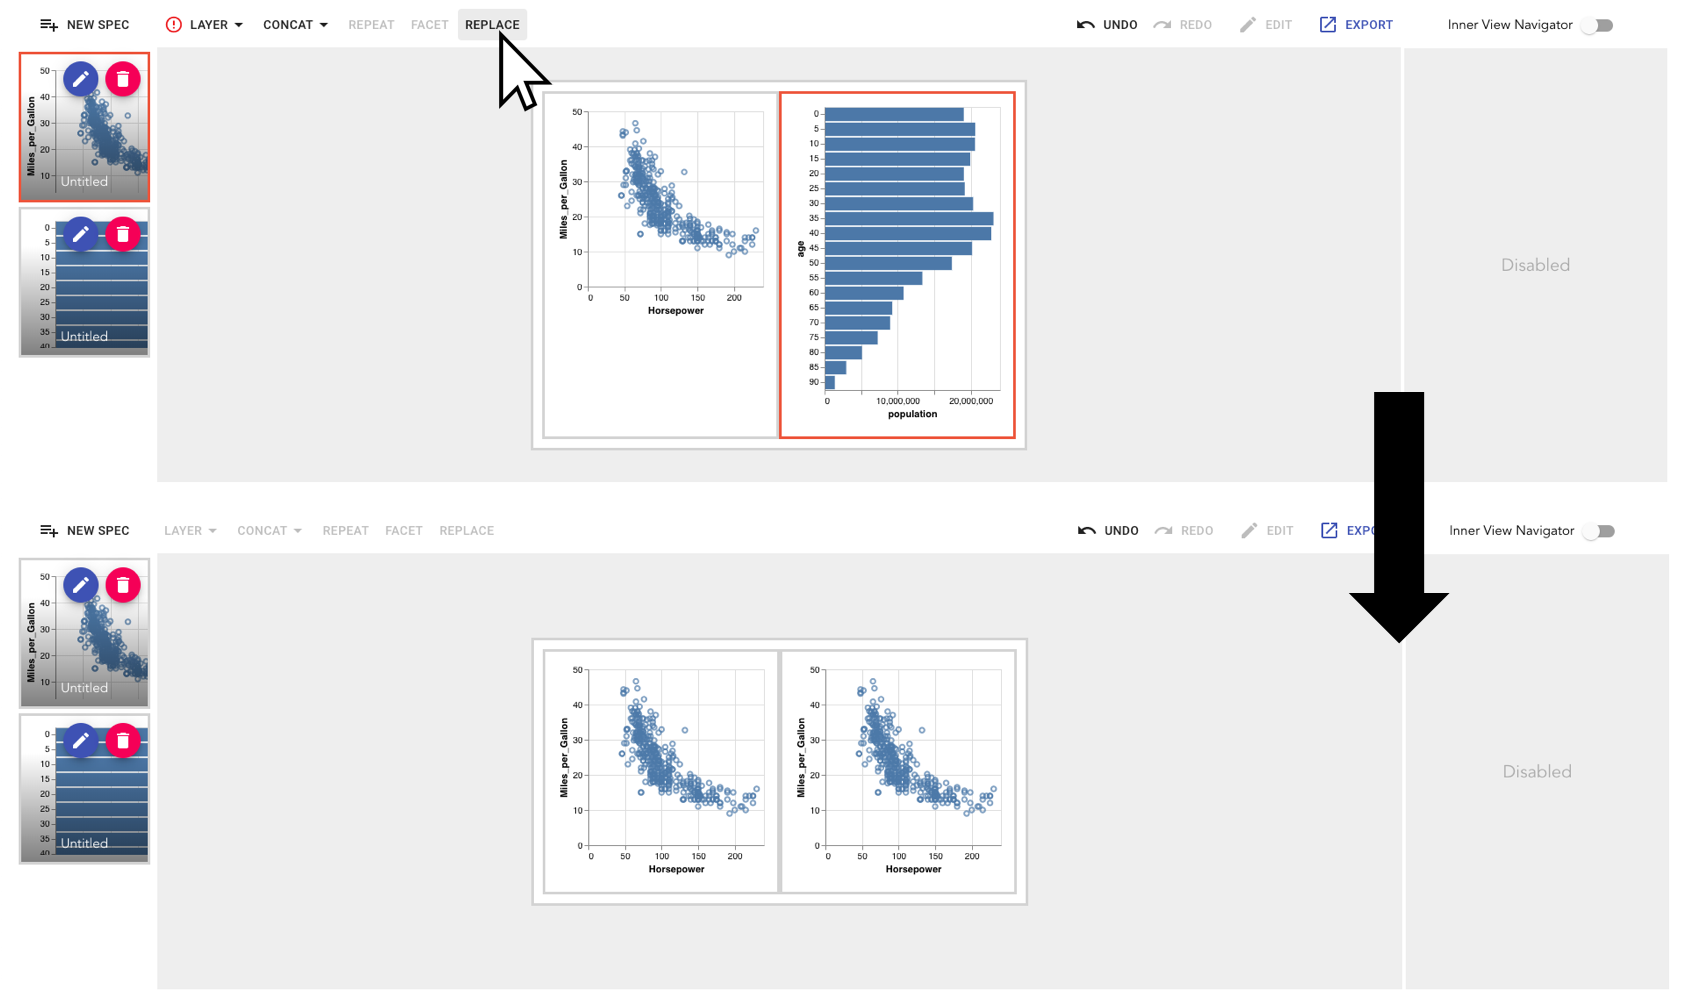
\includegraphics[width=3in]{replace.png}
 \caption{Before and after replacing the selcted bar chart with the selected scatter plot}
\end{figure}

\subsubsection{Layer}
Users can perform layering when there are one selected view from the sidebar and
one selected view from the working area. When clicking “LAYER”, the users are
prompted with an option to layer the view in the sidebar over or under the view
in the working area. Then, the selected view in the working area is layered with
the selected view in the sidebar.

\paragraph{Validation} Layering in Pleiades has some restrictions. First, both
operands for layering has to be either unit views or layer views because
Vega-Lite only allows layering unit and layer specs. Pleiades also perform an
additional check axes compatibility of operands. Then, It will give a warning
in the operation button to let the user know that layering can be done between
these two operands but not fully compatible.

\paragraph{Editing} Users can edit a layer view by selecting the view in the
working area. Then, click “EDIT”. The supported editing functionalities for layer
view are to remove inner views and rearrange the layering order.

\begin{figure}[htb]
 \centering
 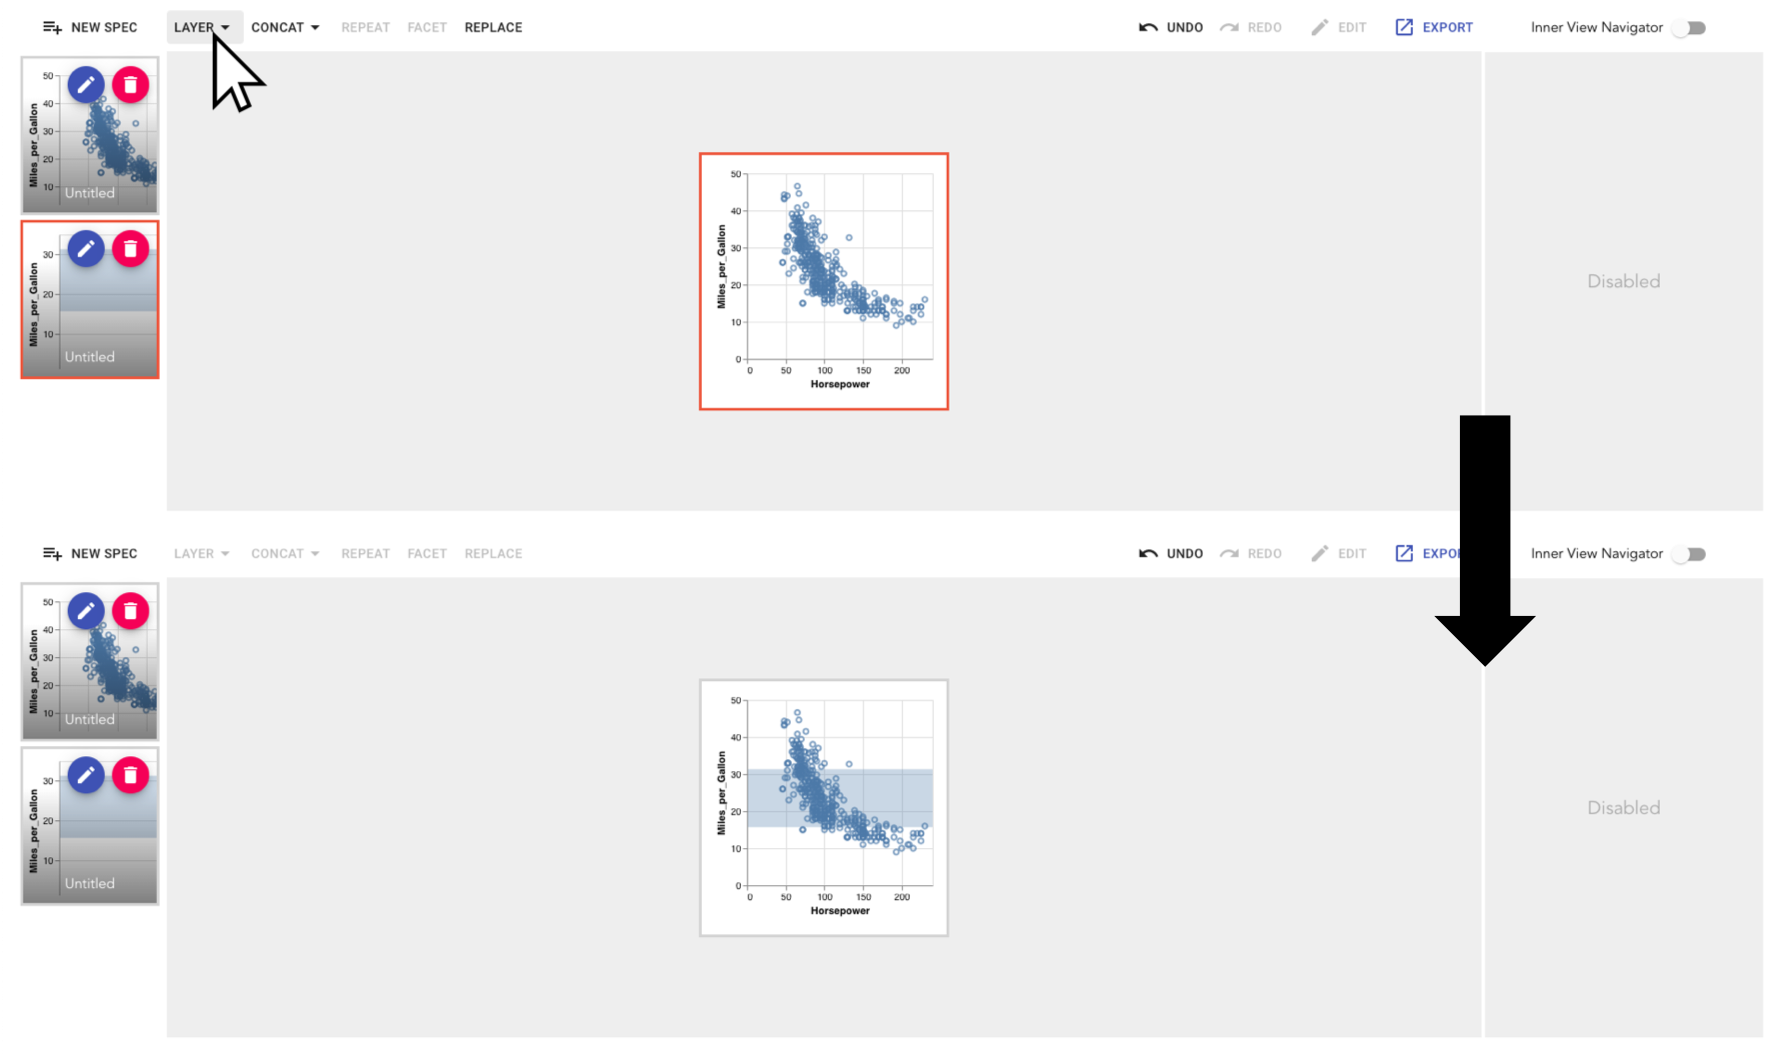
\includegraphics[width=3in]{layer.png}
 \caption{Before and after layering the selcted error-band chart with the selected scatter plot}
\end{figure}

\begin{figure}[htb]
 \centering
 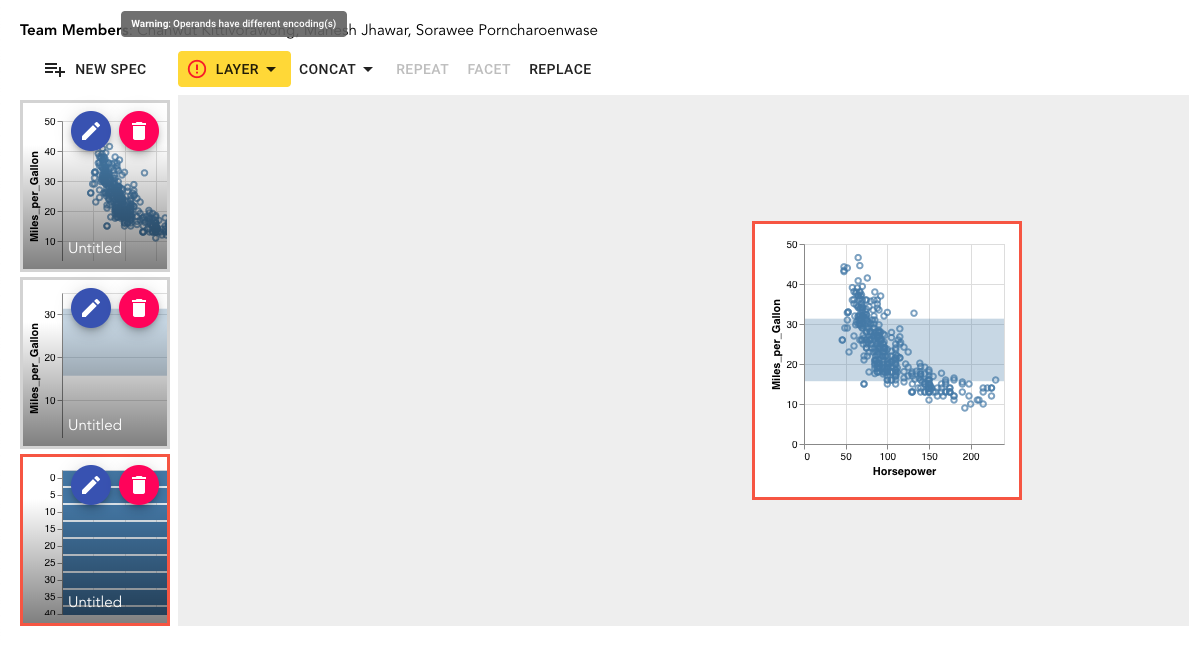
\includegraphics[width=3in]{layer_warn.png}
 \caption{Warning when axes of layering views are not fully compatible (between the bar chart and the scatter plot)}
\end{figure}

\subsubsection{Concatenation}
The user can perform concatenation when there is one selected view from the sidebar
and one selected view from the working area. When clicking “CONCAT”, the user is
prompted with an option to concatenate the selected view in the sidebar to the
left, right, top, or bottom of the selected view in the working area.

\paragraph{Editing} Users can edit a concat view by selecting the view in the
working area. Then, click “EDIT”. In the edit popup window, the user can rearrange
the order of concatenation, remove inner views, and switch between vertical and
horizontal concatenation.

\begin{figure}[htb]
 \centering
 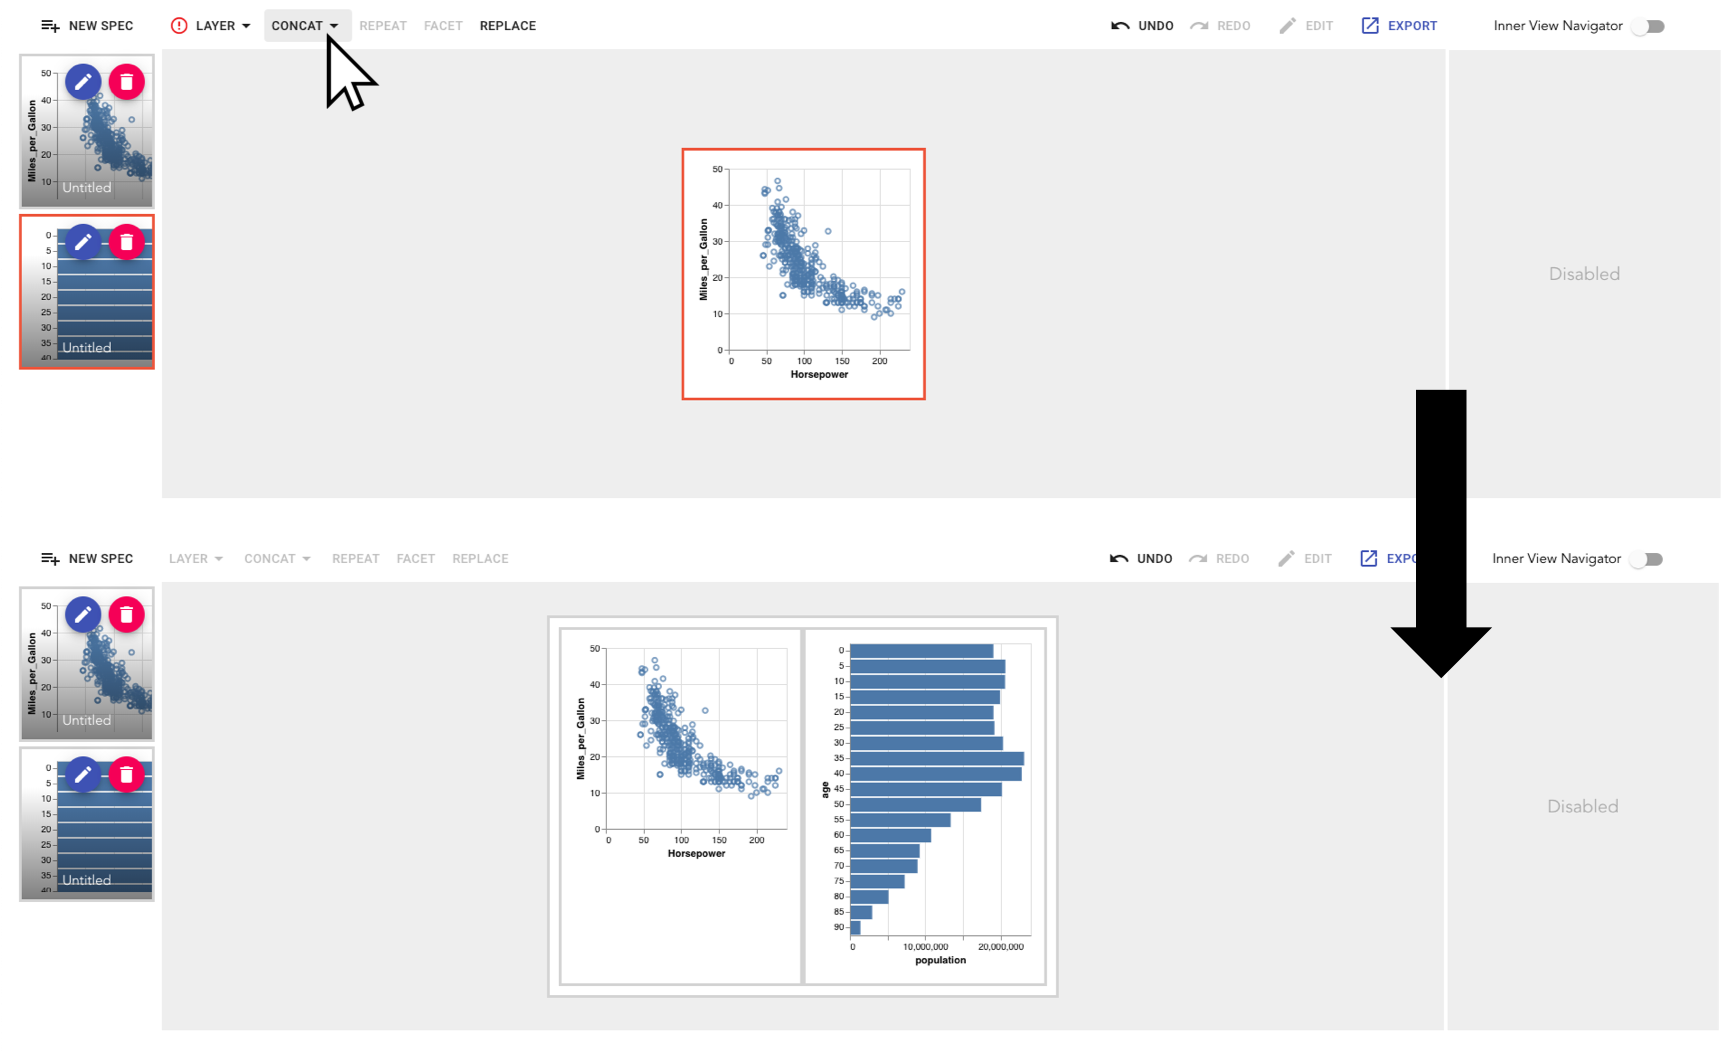
\includegraphics[width=3in]{concat.png}
 \caption{Before and after concatenating the selcted bar chart with the selected scatter plot}
\end{figure}

\subsubsection{Facet}
The user can perform faceting when there is one selected view from the working
area. When clicking “FACET”, a popup window will show prompting the user to select,
for each repeating direction (row or column or both), a field and its type to facet.
Note that facet-ing will be applied to all inner views of the operand. Due to our time
constraints, selecting a subset of inner views to only perform facet on the set of
inner views is unavailable right now.

\paragraph{Validation} Since parameters for facet are fields, facet-ing
depends on the dataset. Thus, “FACET” button will show a warning signal when the
operand has multiple data source. For instance, selecting a concat view that
contains a chart from cars dataset and population dataset will result in having
the warning signal in the “FACET”  button.

\paragraph{Editing} There are two methods of modifying a facet view. Users can
edit the properties of a facet view by selecting the editing view. Then, click
“EDIT”. A popup window will show. Users can change the facet parameters for the
facet view. An option for decompose facet view is also provided to replace the
current facet view with its inner view (the original view). Another method for
modifying a facet view is to modify the inner view of the facet view in the Inner
View Navigator. When selecting a facet view, the inner view of the facet view will
show up in the Inner View Navigator. Then, the user can perform modification to the
view in Inner View Navigator. This modification, however, does not perform any
validation on the datasets, due to the time constraints. If a new view is added
and might break the well-formedness of the state. In practice, this is not a problem
because Pleiades supports undo and redo, so users can always go back to the previous
state when the output is invalid resulting from this modification.

\begin{figure}[htb]
 \centering
 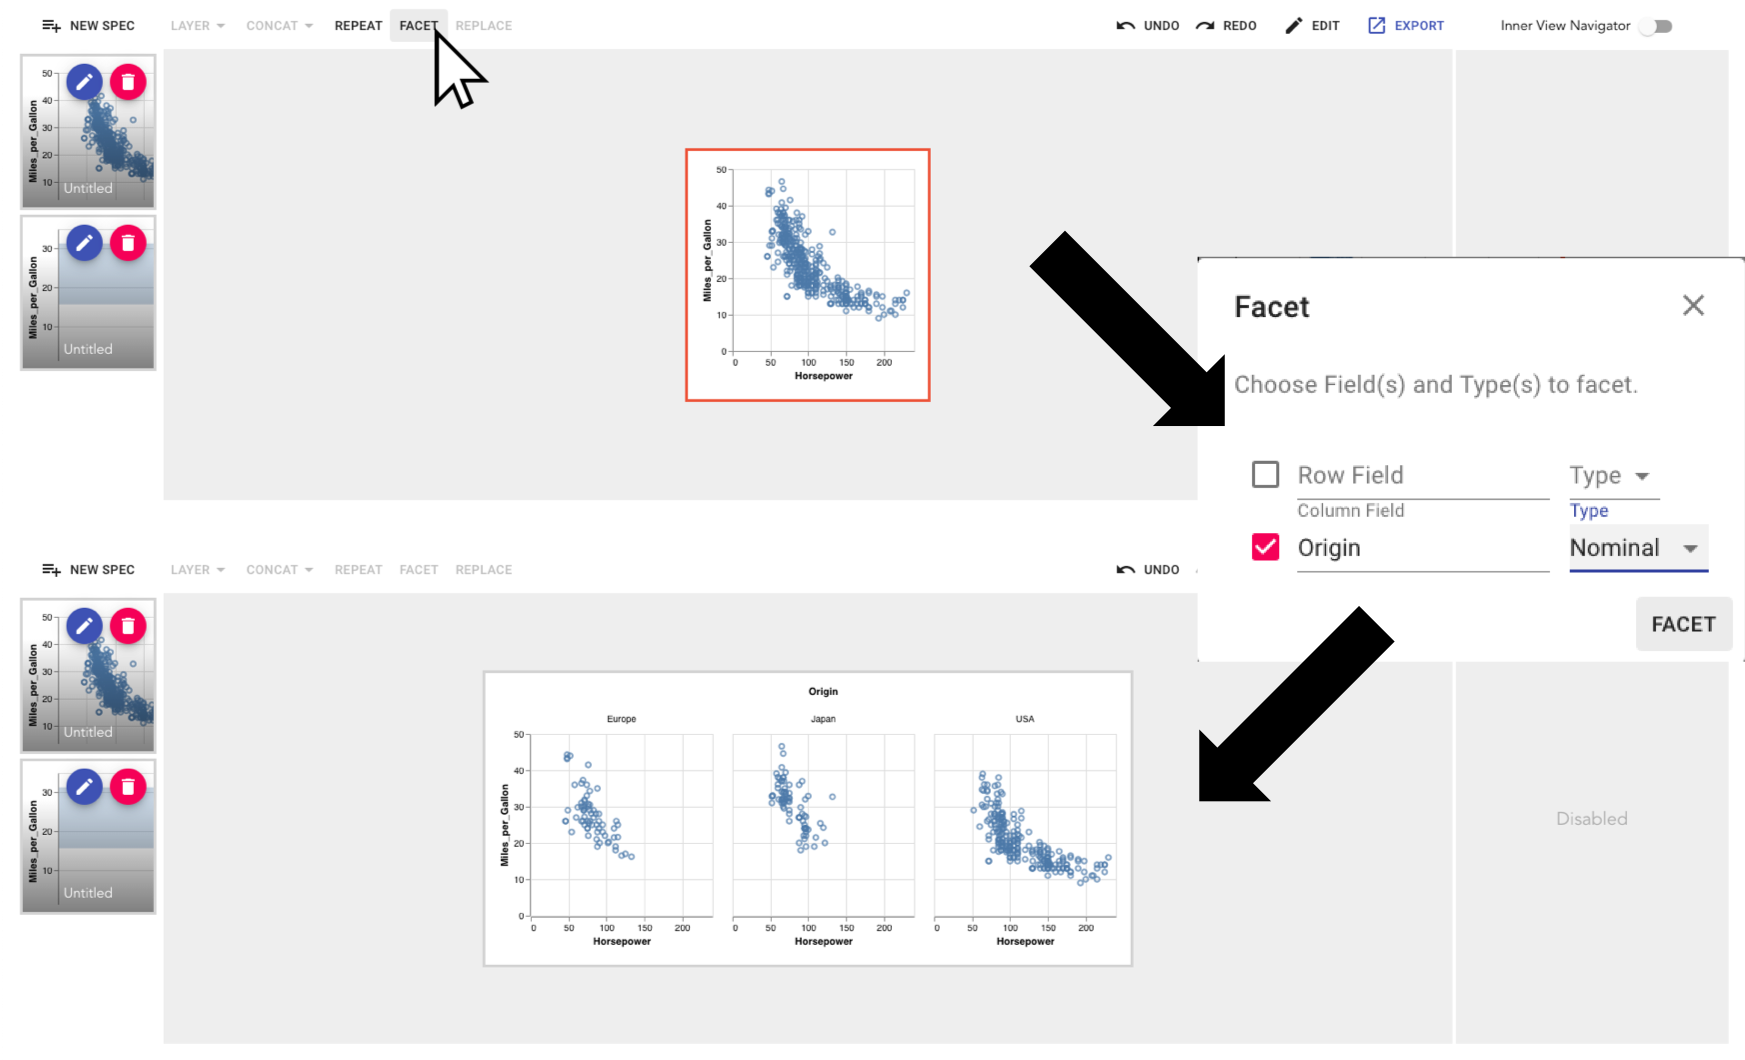
\includegraphics[width=3in]{facet.png}
 \caption{Before and after facet-ing the selected scatter plot with ``Origin'' as the field for facet-ing column.}
\end{figure}

\begin{figure}[htb]
 \centering
 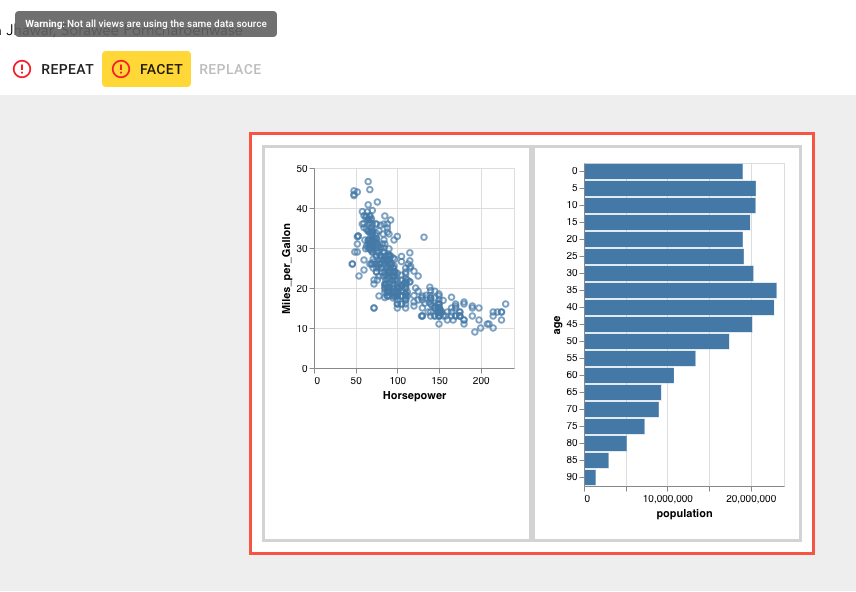
\includegraphics[width=3in]{facet_warn.png}
 \caption{Warning on repeat and facet when not every dataset in the selected view are from the same source.}
\end{figure}

\subsubsection{Repeat}
Every interaction in repeat operation works the same way as it would work in
facet operation with the exception of the operation button to “REPEAT” and the
popup window to configure parameter to perform repeat. The popup window will prompt
the user to input, for each repeating direction (row or column or both), a list of
fields to repeat and encoding channel to repeat. Repeating will also be applied to
all inner views of the operand as same as faceting.

\paragraph{Validation} Repeat operation performs the same validation as the facet
operation does.

\paragraph{Editing} Users can edit repeat view with the same methods as editing facet view.

\begin{figure}[htb]
 \centering
 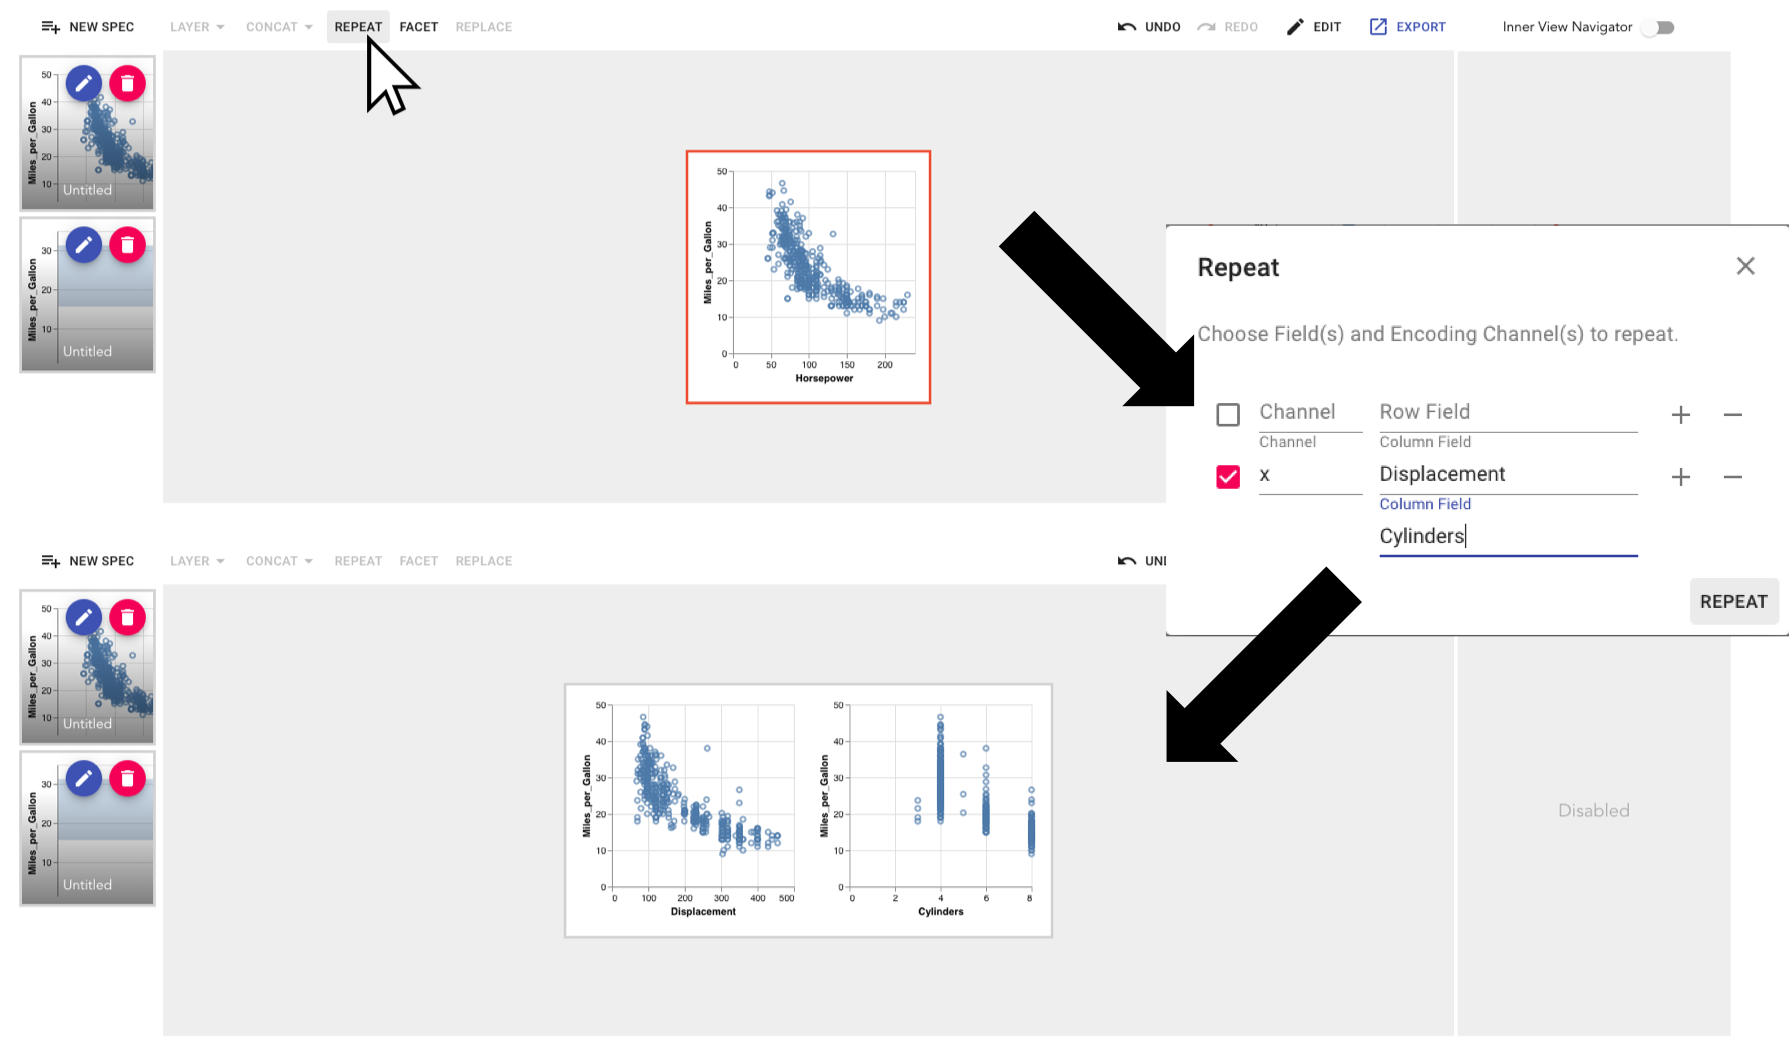
\includegraphics[width=3in]{repeat.png}
 \caption{Before and after repeating the selected scatter plot with ``Displacement'' and ``Cylinders'' as the list of fields for repeat column on x-axis.}
\end{figure}

\subsection{Well-Formedness}
As mentioned, Pleiades will restrict users from performing some operations that
make views incompatible. More broadly, our design goal is that the working area
should be well-formed throughout user interactions, where the working area is
well-formed if it can be exported into a Vega-Lite spec. This might sound difficult
to achieve, but the induction principle gives us a way to decompose the goal into
subtasks: we only need to make sure that every Pleiades’ operation preserves
well-formedness. As the initial view is trivially well-formed, by the induction
principle, it follows that the working area will be well-formed at any time.

The benefit of ensuring well-formedness at every step is that users will never
need to correct a mistake. This contrasts with a tool that allows an ill-formed
state because users then need to find mistakes, which could potentially be anywhere,
and then fix them to make the state become well-formed. Without a good error reporting
system that accurately guides users to fix problems, this process would be very time
consuming and frustrating to users. A good error reporting system, however, is
notoriously difficult to achieve. By ensuring well-formedness at every step, we
can greatly simplify the system while providing good user experience.

To implement well-formedness preserving operations, we perform speculation for
each operation to validate if the operation should be permitted or not. There
are two design decisions that we could make here: one is allowing users to attempt
the operation, which will immediately fail, and the other is disallowing users
from attempting the operation in the first place. The first approach has the advantage
that the error messages could be very descriptive, allowing users to understand
why the operation is not allowed. However, this comes with the cost of a more
confusing user interface. We thus opt for the second approach which disallows
users from attempting the operation in the first place. To mitigate the problem
that users might not understand why an operation is not allowed, we additionally
insert short text to explain why the operation is disabled for some potentially
confusing operations. For example, when the user selects operands to layer, if
one of the operands is not a unit spec or layer spec, the “LAYER” button is
disabled. And if both operands do not have compatible axes, the “LAYER” button
will show a warning sign with a tooltip that the axes are not compatible.

In practice, the above approach is proven to be too rigid. One example of
unintended consequences of the above approach is that users can’t edit any
specification at all, because, during the editing, it’s very likely that
the text won’t be able to parse correctly into the JSON format. We thus
separate operations into macro-operations and micro-operations, where a
macro-operation is a group of micro-operations. We then relax our goal to
only apply to macro-operations. That is, every macro-operation preserves
well-formedness. For micro-operations that does not preserve well-formedness,
the operation won’t affect the working area directly. Rather, it is confined
inside a dialog box so that a batch of micro-operations can be readily reversed.

\subsection{Syntax Tree}
The state of the composite view for the output in the working area is internally
stored as a tree. Each node of the tree represents a view composition, which has
different properties depending on the type of composition.

\subsubsection{UnitView} contains a Vega-Lite specification. However, Pleiades does
not perform any validation to check if the specification is actually a Vega-Lite’s
UnitSpec. So, UnitView can be layer, concat, repeat, or facet spec but cannot be
modified by Pleiades’ operations.

\subsubsection{LayerView} has a list of children nodes representing inner views that
are being layered. The children are only allowed to be UnitView or LayerView.
More specifically, the specification of the UnitView child has also to be either
unit or layer spec as Vega-Lite only allows layering layer and unit specs.

\subsubsection{ConcatView} has a list of children node representing inner views that
are being concatenated and a type of concatenation to be either horizontal or
vertical concatenation. The children of ConcatView can be any type of View.

\subsubsection{FacetView} has one inner view and facet properties, which contains
field and type of row facet and/or field and type of column facet. The inner
view can be any type of Views. All the datasets in the inner view should come
from the same source if the inner view is a composite view. Although Pleiades
does not prevent users from facet-ing View that contains multiple data sources,
it gives a warning to the users that the datasets are not compatible.

\subsubsection{RepeatView} has one inner view and repeat properties, which contains
a list of fields and encoding channel of row repeat and/or a list of fields and
encoding channel of column repeat. Everything else of RepeatView is the same as
FacetView.

\paragraph{The benefit of using syntax tree} With the syntax tree, inner views
can be located to modify easily. Furthermore, when the working view is output to
the working area, it can be rendered recursively through each node in the tree.
This recursive rendering allows us to render inner views as separate views from
the outer view. For example, when rendering concat view, the inner views are
rendered separately in a way that users can select either the inner view or
the whole concat view.

\subsection{How data of each spec is pulled to the top level in facet and repeat}
In facet and repeat spec, data must be at the topmost level of the output JSON
spec. When RepeatView or FacetView is exported to JSON, Pleiades pull out all
the data source in every children view of the inner view to the top level. If
there is more than one distinct data source, Pleiades will use the first one it
encounters by pre-order tree traversal. Pleiades also uses a similar method to
exhaustively search for every data source in the inner views of an operand to
validate if there should be a warning shown for the current operand for facet/repeat.

\section{Results}

The key result for Pleiades was how easy it became to compose graph. 
During our presentation, we asked a lot of our peers to try out our 
application and compare their workflow to that when they used the 
Vega-Lite API along with a JSON spec. The results were as we expected: Pleiades 
gives a better understanding and ease at composing different charts and see
what fits the best. The key-idea behind why Pleiades makes composing charts 
easier and more intuitive is because the process is bottom-up, 
whereas Vega-lite is top-down. Also, the graphical user interface 
provided used with a smother way to compose charts, than to write nested JSON specs. 

One more results that we found was, having the ability to perform 
the four operations: Layer, Concat, Facet and Repeat, it gave the user
a better understanding of these operations and how to properly use then. 
he validation steps, along with the error message that Pleiades provides 
helps users to understand what they are doing wrong, helping them in their 
education about visualization in general. 

In terms of exploring data, the time it takes to compose different 
charts and see find useful results, went down by a lot because of the 
high-level of interactivity provided. Users don’t have to worry about 
updating JSON code for every small change in their chart.

Overall, Pleiades resulted in easing beginners to develop composite 
charts, save time for users, ease data-exploration, and act as a 
support toolkit for education. 


\section{Discussion}

discussion here

\section{Future Work}
We are currently working on extending our software to perform a better validation
of every operation. This validation is important for the software because the
software can then maintain the well-formedness of the output at every state after
every operation. In the current build of the software, we decided to left out some
validations due to the time constraints. However, in the real scenario, not validating
everything is not a problem since our software support undo and redo that users
can always reverse back to the previous state.

As observed from users using Pleiades, users try dragging view to the main view
first when first trying the software. As an extension to Pleiades, we are looking
forward to supporting dragging and dropping in the software to provide a more natural
interaction to the users.

When adding a new spec to the sidebar in the software, Pleiades interpret the new
View as a UnitView regardless of its actual composite type. While this does not
create a problem in practice, the rendered view is always static. For instance,
the inner views of concat spec that is added by “NEW SPEC” are not selectable by
users, and cannot be edited using the “EDIT” button.  Our future work for addressing
this issue is that we would incorporate a parser that parses new specs to syntax tree
of composite views so that all the functionality is supported for the composite
views added by users.

%% if specified like this the section will be committed in review mode
\acknowledgments{
The authors wish to thank A, B, C. This work was supported in part by
a grant from XYZ.}

\bibliographystyle{abbrv}
%%use following if all content of bibtex file should be shown
%\nocite{*}
\bibliography{template}
\end{document}
